
\documentclass[letterpaper,hide notes,xcolor={table,svgnames},pdftex]{beamer}
\def\showexamples{t}


%\usepackage[svgnames]{xcolor}

%% Demo talk
%\documentclass[letterpaper,notes=show]{beamer}

\usecolortheme{crane}
\setbeamertemplate{navigation symbols}{}

\usetheme{MyPittsburgh}
%\usetheme{Frankfurt}

%\usepackage{tipa}

\usepackage{hyperref}
\usepackage{graphicx,xspace}
\usepackage[normalem]{ulem}

\newcommand\SF[1]{$\bigstar$\footnote{SF: #1}}



\newcounter{tmpnumSlide}
\newcounter{tmpnumNote}

% old question code
%\newcommand\question[1]{{$\bigstar$ \small \onlySlide{2}{#1}}}
% \newcommand\nquestion[1]{\ifdefined \presentationonly \textcircled{?} \fi \note{\par{\Large \textbf{?}} #1}}
% \newcommand\nanswer[1]{\note{\par{\Large \textbf{A}} #1}}


 \newcommand\mnote[1]{%
   \addtocounter{tmpnumSlide}{1}
   \ifdefined\showcues {~\tiny\fbox{\arabic{tmpnumSlide}}}\fi
   \note{\setlength{\parskip}{1ex}\addtocounter{tmpnumNote}{1}\textbf{\Large \arabic{tmpnumNote}:} {#1\par}}}

\newcommand\mmnote[1]{\note{\setlength{\parskip}{1ex}#1\par}}

%\newcommand\mnote[2][]{\ifdefined\handoutwithnotes {~\tiny\fbox{#1}}\fi
% \note{\setlength{\parskip}{1ex}\textbf{\Large #1:} #2\par}}

%\newcommand\mnote[2][]{{\tiny\fbox{#1}} \note{\setlength{\parskip}{1ex}\textbf{\Large #1:} #2\par}}

\newcommand\mquestion[2]{{~\color{red}\fbox{?}}\note{\setlength{\parskip}{1ex}\par{\Large \textbf{?}} #1} \note{\setlength{\parskip}{1ex}\par{\Large \textbf{A}} #2\par}\ifdefined \presentationonly \pause \fi}

\newcommand\blackboard[1]{%
\ifdefined   \showblackboard
  {#1}
  \else {\begin{center} \fbox{\colorbox{blue!30}{%
         \begin{minipage}{.95\linewidth}%
           \hspace{\stretch{1}} Some space intentionally left blank; done at the blackboard.%
         \end{minipage}}}\end{center}}%
         \fi%
}



%\newcommand\q{\tikz \node[thick,color=black,shape=circle]{?};}
%\newcommand\q{\ifdefined \presentationonly \textcircled{?} \fi}

\usepackage{listings}
\lstset{%
  keywordstyle=\bfseries,
  aboveskip=15pt,
  belowskip=15pt,
  captionpos=b,
  identifierstyle=\ttfamily,
  escapeinside={(*@}{@*)},
  stringstyle=\ttfamiliy,
  frame=lines,
  numbers=left, basicstyle=\scriptsize, numberstyle=\tiny, stepnumber=0, numbersep=2pt}

\usepackage{siunitx}
\newcommand\sius[1]{\num[group-separator = {,}]{#1}\si{\micro\second}}
\newcommand\sims[1]{\num[group-separator = {,}]{#1}\si{\milli\second}}
\newcommand\sins[1]{\num[group-separator = {,}]{#1}\si{\nano\second}}
\sisetup{group-separator = {,}, group-digits = true}

%% -------------------- tikz --------------------
\usepackage{tikz}
\usetikzlibrary{positioning}
\usetikzlibrary{arrows,backgrounds,automata,decorations.shapes,decorations.pathmorphing,decorations.markings,decorations.text}

\tikzstyle{place}=[circle,draw=blue!50,fill=blue!20,thick, inner sep=0pt,minimum size=6mm]
\tikzstyle{transition}=[rectangle,draw=black!50,fill=black!20,thick, inner sep=0pt,minimum size=4mm]

\tikzstyle{block}=[rectangle,draw=black, thick, inner sep=5pt]
\tikzstyle{bullet}=[circle,draw=black, fill=black, thin, inner sep=2pt]

\tikzstyle{pre}=[<-,shorten <=1pt,>=stealth',semithick]
\tikzstyle{post}=[->,shorten >=1pt,>=stealth',semithick]
\tikzstyle{bi}=[<->,shorten >=1pt,shorten <=1pt, >=stealth',semithick]

\tikzstyle{mut}=[-,>=stealth',semithick]

\tikzstyle{treereset}=[dashed,->, shorten >=1pt,>=stealth',thin]

\usepackage{ifmtarg}
\usepackage{xifthen}
\makeatletter
% new counter to now which frame it is within the sequence
\newcounter{multiframecounter}
% initialize buffer for previously used frame title
\gdef\lastframetitle{\textit{undefined}}
% new environment for a multi-frame
\newenvironment{multiframe}[1][]{%
\ifthenelse{\isempty{#1}}{%
% if no frame title was set via optional parameter,
% only increase sequence counter by 1
\addtocounter{multiframecounter}{1}%
}{%
% new frame title has been provided, thus
% reset sequence counter to 1 and buffer frame title for later use
\setcounter{multiframecounter}{1}%
\gdef\lastframetitle{#1}%
}%
% start conventional frame environment and
% automatically set frame title followed by sequence counter
\begin{frame}%
\frametitle{\lastframetitle~{\normalfont(\arabic{multiframecounter})}}%
}{%
\end{frame}%
}
\makeatother

\makeatletter
\newdimen\tu@tmpa%
\newdimen\ydiffl%
\newdimen\xdiffl%
\newcommand\ydiff[2]{%
    \coordinate (tmpnamea) at (#1);%
    \coordinate (tmpnameb) at (#2);%
    \pgfextracty{\tu@tmpa}{\pgfpointanchor{tmpnamea}{center}}%
    \pgfextracty{\ydiffl}{\pgfpointanchor{tmpnameb}{center}}%
    \advance\ydiffl by -\tu@tmpa%
}
\newcommand\xdiff[2]{%
    \coordinate (tmpnamea) at (#1);%
    \coordinate (tmpnameb) at (#2);%
    \pgfextractx{\tu@tmpa}{\pgfpointanchor{tmpnamea}{center}}%
    \pgfextractx{\xdiffl}{\pgfpointanchor{tmpnameb}{center}}%
    \advance\xdiffl by -\tu@tmpa%
}
\makeatother
\newcommand{\copyrightbox}[3][r]{%
\begin{tikzpicture}%
\node[inner sep=0pt,minimum size=2em](ciimage){#2};
\usefont{OT1}{phv}{n}{n}\fontsize{4}{4}\selectfont
\ydiff{ciimage.south}{ciimage.north}
\xdiff{ciimage.west}{ciimage.east}
\ifthenelse{\equal{#1}{r}}{%
\node[inner sep=0pt,right=1ex of ciimage.south east,anchor=north west,rotate=90]%
{\raggedleft\color{black!50}\parbox{\the\ydiffl}{\raggedright{}#3}};%
}{%
\ifthenelse{\equal{#1}{l}}{%
\node[inner sep=0pt,right=1ex of ciimage.south west,anchor=south west,rotate=90]%
{\raggedleft\color{black!50}\parbox{\the\ydiffl}{\raggedright{}#3}};%
}{%
\node[inner sep=0pt,below=1ex of ciimage.south west,anchor=north west]%
{\raggedleft\color{black!50}\parbox{\the\xdiffl}{\raggedright{}#3}};%
}
}
\end{tikzpicture}
}


%% --------------------

%\usepackage[excludeor]{everyhook}
%\PushPreHook{par}{\setbox0=\lastbox\llap{MUH}}\box0}

%\vspace*{\stretch{1}

%\setbox0=\lastbox \llap{\textbullet\enskip}\box0}

\setlength{\parskip}{\fill}

\newcommand\noskips{\setlength{\parskip}{1ex}}
\newcommand\doskips{\setlength{\parskip}{\fill}}

\newcommand\xx{\par\vspace*{\stretch{1}}\par}
\newcommand\xxs{\par\vspace*{2ex}\par}
\newcommand\tuple[1]{\langle #1 \rangle}
\newcommand\code[1]{{\sf \footnotesize #1}}
\newcommand\ex[1]{\uline{Example:} \ifdefined \presentationonly \pause \fi
  \ifdefined\showexamples#1\xspace\else{\uline{\hspace*{2cm}}}\fi}

\newcommand\ceil[1]{\lceil #1 \rceil}


\AtBeginSection[]
{
   \begin{frame}
       \frametitle{Outline}
       \tableofcontents[currentsection]
   \end{frame}
}



\pgfdeclarelayer{edgelayer}
\pgfdeclarelayer{nodelayer}
\pgfsetlayers{edgelayer,nodelayer,main}

\tikzstyle{none}=[inner sep=0pt]
\tikzstyle{rn}=[circle,fill=Red,draw=Black,line width=0.8 pt]
\tikzstyle{gn}=[circle,fill=Lime,draw=Black,line width=0.8 pt]
\tikzstyle{yn}=[circle,fill=Yellow,draw=Black,line width=0.8 pt]
\tikzstyle{empty}=[circle,fill=White,draw=Black]
\tikzstyle{bw} = [rectangle, draw, fill=blue!20, 
    text width=4em, text centered, rounded corners, minimum height=2em]
    
    \newcommand{\CcNote}[1]{% longname
	This work is licensed under the \textit{Creative Commons #1 3.0 License}.%
}
\newcommand{\CcImageBy}[1]{%
	\includegraphics[scale=#1]{creative_commons/cc_by_30.pdf}%
}
\newcommand{\CcImageSa}[1]{%
	\includegraphics[scale=#1]{creative_commons/cc_sa_30.pdf}%
}
\newcommand{\CcImageNc}[1]{%
	\includegraphics[scale=#1]{creative_commons/cc_nc_30.pdf}%
}
\newcommand{\CcGroupBySa}[2]{% zoom, gap
	\CcImageBy{#1}\hspace*{#2}\CcImageNc{#1}\hspace*{#2}\CcImageSa{#1}%
}
\newcommand{\CcLongnameByNcSa}{Attribution-NonCommercial-ShareAlike}

\newenvironment{changemargin}[1]{% 
  \begin{list}{}{% 
    \setlength{\topsep}{0pt}% 
    \setlength{\leftmargin}{#1}% 
    \setlength{\rightmargin}{1em}
    \setlength{\listparindent}{\parindent}% 
    \setlength{\itemindent}{\parindent}% 
    \setlength{\parsep}{\parskip}% 
  }% 
  \item[]}{\end{list}} 




\title{Lecture 33 --- Software Communication Patterns}

\author{Jeff Zarnett \\ \small \texttt{jzarnett@uwaterloo.ca}}
\institute{Department of Electrical and Computer Engineering \\[-1ex]
  University of Waterloo}
\date{\today}


\begin{document}

\begin{frame}
  \titlepage
\end{frame}

\begin{frame}
\frametitle{Software Communication Patterns}

\begin{changemargin}{1cm}
Software Architecture, Continued.

We will now look at communication architectures:\\
\quad how messages and data are passed.
\end{changemargin}
\end{frame}

\begin{frame}
\frametitle{Pipes and Filters Architecture}

\begin{changemargin}{1cm}
Two major components: pipes and filters.

\emph{Pipe}: Takes input, performs some action, and outputs result.

Take one input, do one thing, produce one output.

\emph{Filter}: Examines input and will either accept it or reject it.\\
\quad Accept: let the data pass and appear in the output.\\
\quad Reject: block the data; no output appears.

\end{changemargin}
\end{frame}

\begin{frame}
\frametitle{Pipes and Filters Architecture}

\begin{changemargin}{1cm}
Example: input messages are formatted with CRLF.

Data will be sent to a system that recognizes only LF as the end of line and considers CR to be an error.

Solution: create a pipe that removes the CR characters.

Alternative: create a filter. Reject messages with CR.

\end{changemargin}
\end{frame}

\begin{frame}
\frametitle{Pipes and Filters Architecture}

\begin{changemargin}{1cm}
Pipes do not have to transform data.

Might have a logging pipe.

Filters are read-only; they do not change data.

\end{changemargin}
\end{frame}

\begin{frame}
\frametitle{Pipes and Filters Architecture}

\begin{changemargin}{1cm}
Pipes and filters can be assembled into a \emph{Pipeline}.

Data enters at the start of the pipeline and passes through the pipes and filters until it gets to the end.

Filters can be at any point.

If a filter rejects a piece of data, it does not advance.

Build a complex system by assembling smaller components.


\end{changemargin}
\end{frame}

\begin{frame}
\frametitle{Pipes and Filters Architecture}

\begin{changemargin}{1cm}
Individual elements are small and simple.

Many components in a system - hidden dependencies?

Not much room for decision-making in processing.

\end{changemargin}
\end{frame}

\begin{frame}
\frametitle{Pipes and Filters Architecture}

\begin{changemargin}{1cm}
Sometimes a third element: \emph{valve}.

Valves are 1 input : 1+ outputs.\\
\quad (Pipes are 1 input : 1 output.)

A way to decide farther down how to proceed.

Example: send the message via e-mail or instant message.

\end{changemargin}
\end{frame}

\begin{frame}
\frametitle{Pipes and Filters Example}

\begin{changemargin}{1cm}
We have a system that accepts XML data within a ZIP file and delivers the extracted XML to a server.

A pipeline for such a system might be written like this:

validZIPFileFilter/extractFromZIPFilePipe/\\
loggingPipe/removeCRPipe/syntaxFilter/deliverToServerPipe


A slash indicates separation between segments of the pipeline.


\end{changemargin}
\end{frame}

\begin{frame}
\frametitle{Pipes and Filters Example}

\begin{changemargin}{1cm}
This example has four pipes and two filters.

\begin{itemize}
	\item \textbf{validZIPFileFilter} \mnote{Rejects any input which is not a valid ZIP file.}
	\item \textbf{extractFromZIPFilePipe} \mnote{Extracts the data from the ZIP file. At this stage we can be sure that we have a ZIP file as the input (and not a plain text or pdf file or something else) because those would have been blocked at the previous stage.}
	\item \textbf{loggingPipe} \mnote{Examines the extracted data and writes some information to the logs. }
	\item \textbf{removeCRPipe} \mnote{As above, removes the Carriage Return characters from the data, if any.}
	\item \textbf{syntaxFilter} \mnote{ Accepts only data which has valid syntax (XML is valid); rejects all others.}
	\item \textbf{deliverToServerPipe} \mnote{ Sends its input to the server via some specified form of communication.}
\end{itemize}


\end{changemargin}
\end{frame}

\begin{frame}
\frametitle{Pipes and Filters Example}

\begin{changemargin}{1cm}
UNIX example: 

The system utilities like \texttt{ls}, \texttt{cat}, and so on are all small and do exactly one thing (like pipes).

On the commandline you can create a pipeline connecting these two or more items.

\texttt{cat lectures.txt | grep blackboard} \mnote{This is actually two different commands linked together in a pipeline. The first command, \texttt{cat}, reads the file \texttt{lectures.txt} and outputs it. If that command were run alone, it would output the text of the file to the console, but instead there is a \texttt{|} pipe symbol after it, which means the output of the \texttt{cat} command is piped to the \texttt{grep} command. The \texttt{grep} command searches its input for occurrences of the word ``blackboard'' and prints as output the lines where the word blackboard is found. Because we did not specify another pipe symbol and another destination, the output of \texttt{grep} appears on the console.}

\end{changemargin}
\end{frame}

\begin{frame}
\frametitle{Blackboard Architecture}

\begin{changemargin}{1cm}
\emph{Blackboard}: Common knowledge base.

Independent agents work on the knowledge base.

Agents co-operate to solve the problem.

\end{changemargin}
\end{frame}

\begin{frame}
\frametitle{Blackboard Architecture Analogy}

\begin{changemargin}{1cm}
Imagine a difficult math problem.\\
\quad To solve it, assemble a group of math professors.

The processors will collaborate using a physical blackboard.

Each watches to see if he/she can apply his/her expertise.

When a professor can contribute, he/she writes on the board.

\end{changemargin}
\end{frame}


\begin{frame}
\frametitle{Blackboard Architecture Analogy}

\begin{changemargin}{1cm}
After writing something, hopefully someone else can now act.

Professors continue contributing until the problem is solved.

But perhaps nobody can proceed; then professors have failed.

\end{changemargin}
\end{frame}

\begin{frame}
\frametitle{Blackboard Architecture}

\begin{changemargin}{1cm}
Three major components in a Blackboard system.

Software agents or \textit{Knowledge Sources} (professors).

Blackboard: shared repository of problems \& partial solutions.

Moderator: controls access so agents do not interfere.\\
	\quad (Moderator stops profs from fighting over the chalk.)

\end{changemargin}
\end{frame}

\begin{frame}
\frametitle{Blackboard Architecture}

\begin{changemargin}{1cm}
Unusual architecture; few domains where it is best choice.

Usually one agent is best for a problem.

Example: Optical Character Recognition (OCR).

Example: Artificial Intelligence.

\end{changemargin}
\end{frame}


\begin{frame}
\frametitle{Blackboard Architecture}

\begin{changemargin}{1cm}
Advantage: can solve problems that are otherwise intractable. 

Advantage: might be more efficient or faster.

Disadvantage: complex system, difficult to understand.

Disadvantage: limited applicability.

\end{changemargin}
\end{frame}


\begin{frame}
\frametitle{Publish-Subscribe Architecture}

\begin{changemargin}{1cm}
Message passing system.

The sender of a message is called a \textit{Publisher}. 

The publisher does not know whom the reciever(s) of the message is (are). 

Receivers are called \textit{Subscribers}. 

Subscribers register interest in certain kids of messages without knowledge of any publishers.

\end{changemargin}
\end{frame}

\begin{frame}
\frametitle{Publish-Subscribe Architecture}

\begin{changemargin}{1cm}

There may be a third party involved, called a \textit{Broker}.

Brokers connect the publishers and subscribers indirectly. 

If there is no Broker, any subscriber who is not ``listening'' at the time the message is published will not receive the message. 

Broker is a place where the publisher can publish the message so subscribers can collect the message at their convenience.


\end{changemargin}
\end{frame}

\begin{frame}
\frametitle{Publish-Subscribe Architecture}

\begin{changemargin}{1cm}

Subscribers are usual not interested in all messages.

Two ways to filter, not mutually exclusive:

\textit{Topic-Based}: topics/channels. \mnote{systems have a list of topics, and publishers write in these topics (broadcast on this channel) and subscribers listen to that channel.}\\
\quad Example: ECE~155 topic. \mnote{I create an ECE~155 topic, and students subscribe to it. It is then my responsibility as the sender to identify a message in advance as being part of the ECE~155 topic so it will be published on that channel. }

\textit{Content-Based} content-matching. \mnote{messages are delivered to a subscriber if the content of that message matches what the subscriber is looking for.}\\
\quad Example: any message with the text ``ECE~155''.

Note publisher vs. subscriber filtering responsibility.

\end{changemargin}
\end{frame}

\begin{frame}
\frametitle{Publish-Subscribe Architecture Advantages}

\begin{changemargin}{1cm}

\begin{itemize}
\item No dependency between publishers \& subscribers.
\item Scales well; we can have $m$ publishers \& $n$ subscribers.
\item Broker allows asynchronous communication.
\end{itemize}
\end{changemargin}
\end{frame}

\begin{frame}
\frametitle{Publish-Subscribe Architecture Disdvantages}

\begin{changemargin}{1cm}

\begin{itemize}
\item No certainty a message was delivered.
\item Publishers might assume subscribers are listening even if they are not.
\item Broker can be a central point of failure.
\end{itemize}
\end{changemargin}
\end{frame}

\begin{frame}
\frametitle{Publish-Subscribe Example}

\begin{changemargin}{1cm}
RSS (Really Simple Syndication) feeds use publish-subscribe.

The author publishes his writing on the blog.

Subscribers to the RSS feed get a notification.
 
This new message contains the published content.


\end{changemargin}
\end{frame}

\begin{frame}
\frametitle{Peer-to-Peer Architecture}

\begin{changemargin}{1cm}
Different nodes (computers or programs) in the network both supply and receive resources.

Contrast with client-server model where the client requests resources that the server provides.

Tasks like searching for files or streaming audio/video are shared amongst the interconnected peers.

Peers contribute some resources (e.g., processing power).

No centralized server.

\end{changemargin}
\end{frame}

\begin{frame}
\frametitle{Peer-to-Peer Architecture}

\begin{changemargin}{1cm}
\begin{center}
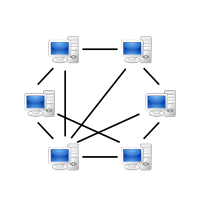
\includegraphics[width=0.35\textwidth]{images/p2pnetwork.png}
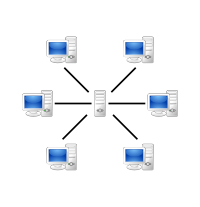
\includegraphics[width=0.35\textwidth]{images/serverbased.png}\\
Left side: A P2P network with a central admin system;\\
Right side: a network based on the client-server model.\\
\texttt{http://en.wikipedia.org/wiki/Peer-to-peer}
\end{center}


\end{changemargin}
\end{frame}

\begin{frame}
\frametitle{Peer-to-Peer Example: Napster}

\begin{changemargin}{1cm}
Napster was a P2P file transfer system, used to share music. 

There was no central repository of music files;\\
\quad each user shared what files he had locally;\\
\quad could browse the files others made available. 

P2P systems are commonly associated with sharing copyrighted material (music, movies);\\
\quad the P2P network is just the form of communication. 

Linux distributions like Ubuntu provide an option to download their installation CDs via BitTorrent.

\end{changemargin}
\end{frame}


\begin{frame}
\frametitle{P2P Advantages \& Disadvantages}

\begin{changemargin}{1cm}
Advantages:
\begin{itemize}
	\item Ability to serve content increases with users.
	\item Decentralized; no single point of failure.
\end{itemize}

Disadvantages:
\begin{itemize}
	\item Communication and search overhead is high.
	\item Co-ordination as peers enter and leave the network.
	\item No guarantee of finding what is sought, even if available.
\end{itemize}

\end{changemargin}
\end{frame}

\begin{frame}
\frametitle{P2P: Distributed Systems}

\begin{changemargin}{1cm}
If peer-to-peer networks are a subject of interest for you, take the class ``Distributed Systems''
\end{changemargin}
\end{frame}



\end{document}
